%!TEX root = ../main.tex
\chapter{Implementation}\label{chapter:implementation}
In this chapter we give a detail explanation of how we implemented and conducted our research as described in~\autoref{chapter:methodology}.
We start with study of old database structure and creation of reverse index in~\autoref{sec:Old Database and Reverse Index}.
We describe the implementation of the \emph{packer} and the \emph{unpacker} to run the candidate pair inside \emph{Anubis} in~\autoref{sec:packerunpacker} and in~\autoref{sec:Initial Experiment} we run our preliminary test of candidate pairs.
Because the old database did not had record of failed activities, we create the new database with both success and failed resource activity in~\autoref{sec:Creation of Database}.
The implementation of LDA based on resource activities from the newly created database is describe in~\autoref{sec:Document Clustering}.
Finally, in~\autoref{sec:Finding Optimal Candidate Pairs}, we describe the use of max-flow approach and heuristics to find the optimal sets of candidate malware pairs corresponding to interesting resource.

\section{Old Database and Reverse Index}
\label{sec:Old Database and Reverse Index}
Our work was based on wide variety of millions of malware samples, collected over the years, by \emph{Anubis}.
% Our main resource for the research was the direct access of the millions of malware samples from Anubis collected over the years in wild.
We had to effectively and efficiently analyze those to find the behavioral interference between malware families.\\
We started with studying the Anubis system and its database.
We primarily dealt with two database of Anubis backend, the \textbf{`db\_report'} and \textbf{'web\_analysis'}.
The \emph{`web\_analysis'} database was hit first for any binary submitted for analysis from public web interface.
Some of the important tables to our work were \emph{`result', `file', and `file\_task'}.
Each submission is a unique row data in \emph{`result'} table.
A new row is also created in \emph{`file'} table with the \emph{`md5'} and \emph{`sha'} hash of the submitted binary.
We refer the unique primary key of the \emph{`file'} table as \textbf{malware id}.
The \emph{file} and \emph{`result'} tables are associated through \emph{`file\_task'} table.
The analysis of the sample would be done for behavioral activities related to different resource types such as File, Registry, and Mutex.
These activities were saved in `\emph{db\_report}' database.
The resource activities of the malware in \emph{`db\_report'} database was associated with the \emph{`web\_analysis'} database by the constraint key \textit{`result\_id'} of the \emph{`result'} table.
In~\autoref{lst:resultidsql}, in the first line, we show a simple \emph{sql} statement to get the \emph{result\_id} and \emph{md5} of the binaries submitted to Anubis from the \emph{`web\_analysis'} database.
In the second line, we get the names of the files created by the binary whose \emph{result\_id} is `\emph{12345}' from the \emph{`db\_report'} database.\\
\begin{lstlisting}[language=sql,caption={sql showing database structure to get file created activities of a malware sample},label={lst:resultidsql}]
SELECT result_id, md5 FROM web_analysis.result join web_analysis.file_task using (task_id) join web_analysis.file using (file_id) WHERE task_id = result_id;
SELECT name from db_report.file_created join db_report.file_name using (file_name_id) where result_id = '12345';
\end{lstlisting}

The total number of malware samples that we had in our test database were \textbf{\gettotalmalwarei{}}.
Initially we considered 3 resource types \textit{File, Registry, Mutex}, and queried the database for \textit{create, read, delete} resource activities.
For each resource type, their \textit{create, read, delete} resource activities were queried.
Our first step was to create a reverse index from the database so that we could get the list of malware that created/deleted/read the resource.
Since, the number of malware to process were in millions, trying to save all their activities in a data structure would cause our machine to run out of memory and crash.
We approached this problem with map reduce technique.\\

We worked on a batch of $50,000$ malware at a time, and saved the reverse index of activity to the file with a numbering for each batch.
The resultant numbered files were in the format where resource name and list of unique malware ids were separated by commas (,) as delimiter.
The numbered files of each resource types were sorted, and then joined, to get the final reverse index.
The sort and join operation is shown in~\autoref{lst:sortandjoin} and was fast as it was a merge sort $O( n \times \log(n))$.
Comma is the field separator for both commands denoted by option \emph{`-t'}  and the operation was done on first field denoted by option \emph{`-k'}, which is the resource name.\\

\begin{lstlisting}[numbers=none,language=bash,caption={Sort and join the reverse index},label={lst:sortandjoin}]
  LANG=en_EN sort -t, -k 1,1 $file_name
  LANG=en_EN join -t , -a1 -a2 $file_name1 $file_name2
\end{lstlisting}

\begin{lstlisting}[numbers=none,caption={Sample of reverse index created for File activity},label={lst:reverseindex}]
C:\mbr.exe,189524063,184501719,87504631,86763863
Buttons,111448211
C:/DOCUME~1/ADMINI~1/LOCALS~1/Temp/telnet.exe,178046895,174206059,183601891,89650247
C:/DOCUME~1/ADMINI~1/LOCALS~1/Temp/1.jpg,161552035,116241803
\end{lstlisting}

A snippet of reverse index of file created activity is shown in~\autoref{lst:reverseindex}, where resource type \emph{`file'}, with resource name \emph{`mbr.exe`}, is created by malware with ids \emph{189524063, 184501719, 87504631, and 86763863}.

From the reverse index of the resource activities of the Malware, we mapped created activities against the deleted or read activities.
% We made a list of malware based on the common resource name as the key, where a list of malware which created the resource and another list of malware which delete/read the same resource.
We started looking for one to one interaction of malware to a single resource.
We looked for a set $(a, b)$, where malware `a' creates the resource \emph{r}, and malware `b' deletes the same resource, \emph{r}, such that no other malware has create or delete activities on that resource \emph{r}. We ran those malware pairs in the Anubis system using the \emph{Unpacker}.
\section{Packer and Unpacker}
\label{sec:packerunpacker}
In order to run the pair of malware together inside the Anubis environment we made a Win32 console application (Anubis uses Windows XP as underlying OS.\@), named \textbf{Unpacker}.
We used the fact that we can append any extraneous data at the end of Windows PE executable, and it would not affect the executable's program flow.
We wrote a \textbf{Packer} program that would add the candidate binary pair at the end of the \emph{Unpacker} binary and then further appends the time delay and file size of each candidate binary as meta information.
The structure of the Unpacker binary is shown in~\autoref{fig:unpacker}.
The \emph{Unpacker} binary, when executed, would read itself from the back to get the meta information and read candidate binaries bytes.
% We created a meta binary, that will read itself, and extract the other two binaries, that will be attached to it.
It will then create the candidate binaries from the read bytes, and run both binaries with a time delay given.\\
\begin{figure}[htbp]
  \centering
  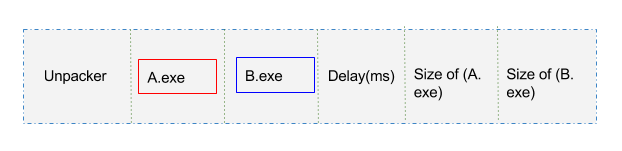
\includegraphics[scale=0.5]{figures/unpacker.png}
\caption{Structure of the Unpacker binary that would create the candidate pair and run them with delay.}
\label{fig:unpacker}
\end{figure}

Code snippet of the \emph{`Unpacker'} binary is shown in~\autoref{lst:unpacker.c}.
We used a struct of 3 integer size to read and hold the meta information. The size of last three \textit{unsigned int} byte of \emph{Unpacker} has the binary pair sizes information and the delay time, known as meta information.
The offset for meta-information was calculated by deduction of $3 \times \textit{size of `uint'}$ from the total size of itself (Unpacker).
We calculate the starting position of appended binaries, and use \texttt{`fseek\(\)'} function to set the file position pointer there.
We then start reading the bytes until the exact size of binary is read.
The read bytes were then saved to create new binary file.
We used \emph{windows.h} standard library's functions: \emph{`CreateProcess'} function to execute the binary, and \emph{`Sleep'} function for delay in between two execution.\\

\begin{lstlisting}[language=c,caption={snippet of Unpacker.c file}, label={lst:unpacker.c}]
  /* stuct for storing meta information */
  typedef struct {
    unsigned int delay;
    unsigned int fsize1;
    unsigned int fsize2;
  }meta_info;

  /* reading the meta information and first binary */
  rfp = fopen(argv[0], "rb");
  wfp1 = fopen(fileName1, "wb");

  fseek(rfp,0,SEEK_END);
  size = ftell(rfp);
  offset = size - sizeof(meta_info);
  fseek(rfp, offset, SEEK_SET);
  fread(&info, 1, sizeof(info), rfp);

  /* calculate the unpackersize from the offset and files size. */
  unpackersize = offset - (info.fsize1 + info.fsize2);

  /* rewind back and to the point of the start of file1 */
  fseek(rfp,0,SEEK_SET);
  fseek(rfp, unpackersize, SEEK_SET);

  nread_sofar = 0;
  while (nread_sofar < info.fsize1) {
      nread = fread(buf, 1, min(info.fsize1 - nread_sofar, sizeof(buf)), rfp);
      nread_sofar += nread;
      fwrite(buf, 1, nread, wfp1);
  }
  fclose(wfp1);
 \end{lstlisting}
\section{Initial Experiment}
\label{sec:Initial Experiment}
During our initial run of candidate pairs, we found lots of dropper malware causing this interaction.
For a candidate pair $(a,b)$, binary `a' was a dropper that would create many binaries including the binary `b', and binary `b' actually read itself upon execution, which was recorded as read activity by Anubis.
After running many other candidate pairs and analyzing the results manually, we were able to understand the Anubis report in depth and also found a logical error on our current approach.\\

Our notion behind checking the malware interaction was finding candidate pairs such that one malware `a' creates some resource, `r', and another malware `b' tries to access or delete the same resource, `r'.
But, Anubis ran each submitted binaries in an isolated environment; hence there was no way that a malware sample `b' would find the resource that was supposed to be created by malware `a'.
We should have been looking for failed attempt activities, where a malware sample unsuccessfully tries to access or delete a resource created by another malware.
But, the current database had no record of such failed attempt.
This lead us to look for the alternatives where we could find log of such failed attempt activities during the execution of binary.\\

We parsed the behavioral profiles, as described in~\autoref{sub:Behavioral Profile}, of malware samples to find failed activities of deletion and access.
\section{Creation of Database}
\label{sec:Creation of Database}
Each malware submitted to Anubis had its own unique behavioral profile saved as python pickle~\cite{pythonpickle} object.
We parsed behavioral profile and extracted the object names and operations from the \emph{OS Object} and \emph{OS Operations} respectively.
The object name is the name of the resource and operation is the activity performed on the resource.
% The OS operation was categorized into \emph{modify}, \emph{access}, and \emph{delete} activity according to the mapping in~\autoref{lbl:ntapi}.
The status of the operation, failed or successful, was taken into account this time.
The resource name, type of operation, and status of operation represented the resource activities of a malware.
We create a new database with resource activities of all our malware samples.\\

We considered eight resource type into account while parsing the profile files: File, Registry, Sync, Section, Process, Service, Job, and Driver [see \autoref{sub:Resource Types and Activities}].
Windows Native and Windows API calls were generalized into OS Operation during the creation of behavioral profile [see~\autoref{sub:Behavioral Profile}].
We went through the list of OS Operations~[\autoref{ssub:OS Operations}] and mapped them into the broad three categories \emph{Modify, Access, and Delete}.
The modify, access, and read list for the resource types \emph{\getresourcetypes{}} are shown in~\autoref{lbl:ntapi}.\\

\begin{lstlisting}[float,floatplacement=ht,numbers=none,language=ruby,caption={Mapping of generalized OS Operation from behavioral profile},label={lbl:ntapi}]
MODIFY_LIST = {
        file:      ["create_named_pipe", "create_mailslot", "create", "rename", "set_information", "write", "flush_buffer", "map"],
        registry:  ["create", "restore_key", "save_key", "set_value", "set_information", "mem_write"],
        process:   ["create", "set_information", "suspend", "resume", "unmap", "map"],
        job:       ["assign", "set_information"],
        driver:    ["unload", "load"],
        section:   ["create", "map", "unmap", "mem_write", "set_information"],
        sync:      ["create", "map", "set_information", "mem_write"],
        service:   ["create", "start", "control"]
        }

ACCESS_LIST = {
        file:      ["query_file", "query", "open", "query_directory", "query_information", "read", "monitor_dir", "query_value"],
        registry:  ["enumerate", "enumerate_value", "monitor_key", "open", "query", "query_value", "mem_read"],
        process:   ["open", "query"],
        job:       ["open", "query"],
        driver:    ["query"],
        section:   ["open", "query", "mem_read", "read", "query_file", "query_system"],
        sync:      ["open", "query"],
        service:   ["open"]
        }

DELETE_LIST = {
        file:      ["delete", "open_truncate"],
        registry:  ["delete", "delete_value"],
        process:   ["delete"],
        job:       ["delete"],
        driver:    ["delete"],
        section:   ["delete"],
        sync:      ["delete"],
        service:   ["delete"]
        }

\end{lstlisting}

% With the resource name, operations and status we create a new database of malware activities.

We used \textbf{MySql Version 5.5.46} as our database engine. MySQL~\cite[]{mysql} is highly scalable and flexible relational database system which complies with the ACID model~\cite[]{acid} design principle.
We used multiple workers to create the database, and ACID compliance prevented from inconsistency of data when being updated across multiple tables.\\

Recreating the database was one of the bottleneck in our project and consumed much time.
The behavioral profile files had to be accessed via network file system.
We need to walk through large list of directories consisting of hundreds of thousands of file, to search the behavioral profile pickle~\cite[]{pythonpickle} of specific malware.
We found \emph{\gettotalmalwareii{}} behavioral profile files out of \emph{\gettotalmalwarei{}} malware.\\

% The basic CRUD operations were time expensive and made the overall operation slow.
While creating the new database, we hit the integer overflow for the primary index key of `\emph{registry access}' table.
We did not anticipate the number of records to cross maximum \emph{`int (10)'} limit \emph{4,294,967,295}.
We created another ``\emph{registry access}' table, with different table name, and start inserting the registry access records in the new table.
When accessing the data for later use, we re-factored our program so that we checked both the registry tables in order to find the registry access activities of a malware sample.\\
% We performed database tuning (buffer size, query cache, threads pool) to increase the speed of database operations.
% We used \emph{cPickle}, which made the reading of pickle file 3 times faster than default python \emph{pickle} module.

We processed \gettotalmalwareii{} behavioral profiles.
The final database size was 1.2 Terabyte.
About $62\%$ of execution time was taken to load the gzip pickle~\cite[]{pythonpickle} of malware profile and the normal SQL CRUD (create, read, update, and delete) operation, which can be seen in Figure~\ref{fig:dbcreation}.\\
% The execution profile is shown in~\autoref{fig:dbcreation}
%TODO: put profile.png
\begin{figure}[ht]
    \centering
    \def\svgwidth{\columnwidth}
    \scalebox{0.99}{\input{figures/dbcreate.pdf_tex}}
    % \input{figures/overview.pdf_tex}
\caption{Profile of new database creation}
\label{fig:dbcreation}
\end{figure}

After the creation of new database, we made a reverse index, like before, for the `\emph{resource name}' to `\emph{malware ids}' modifying, accessing, and deleting the resource.
This time the refined database had both the success and failed resource activities.
% Getting all the resource activities related to all the resource types \emph{file, registry, section, driver, sync,service, process, and job} was also time expensive.
The reverse indexes were used to map resources that were successfully modified with resources that were read/accessed with failed attempt.
For instance, we made a mapping between file successfully modified and failed file deletion, and mapping between file successfully modified and failed file access.
We made same mapping for all other 7 resource types.
All the mapping was done based on the common `\emph{resource name}'.\\

With the reverse index mapping, we chose the candidate pairs such that one malware created the resource and another malware made a failed attempt to delete/access the same resource.
But, the number of possible pairs were too many with this simple heuristic and we hit the \emph{n-combination} problem.
A single resource \texttt{`r'} would have been created by tens of thousands of malware and another tens of thousands of malware trying to access/delete it unsuccessfully.
The combination of candidate pairs from the candidate sets with thousands of malware are of large number to run and analyze result.\\
%TODO: add one more reason "not good enough"

We wanted to filter our candidate sets without compromising the quality.
We performed clustering of the malware based on their resource activities (behavior) to address this problem.
Malware dataset were clustered into different families and candidate pairs were chosen such that they belong to different families.
\section{Document Clustering}
\label{sec:Document Clustering}
Before the clustering, we filtered our malware dataset from the reverse index mapping by removing all resource activity that we confirmed as benign based on our benign list and knowledge.
We sorted the reverse index (resource name to malware ids) with respect to the count of malware ids associated with the resource name in descending order.
With this, we had most commonly modified/accessed/created resource at the top of the list.
We went through the resource name until we found some interesting resource name which does not look benign.
We excluded all benign resources preceding the first interesting suspicious resource name.
For instance, file resource name such as \emph{`Dr.\ Watson.exe'} and \emph{`Sample.exe'} were some resources with highest number of malware interacting with them.
The reasons are \emph{`Dr Watson'} file is created whenever a binary crashes and \emph{Sample.exe} is the name, the submitted binary gets renamed to, by Anubis.
We filtered all such benign resource activities related to resource types {\getresourcetypes{}}.
% Resource types service, job, and driver did not have any interesting mapping.
After the filtering, the total number of malware samples were {\gettotalmalwareiii{}}.\\

We created the text corpora for those {\gettotalmalwareiii{}} malware, and performed the document clustering.
We converted all the resource activities of the malware samples into the corpora text as discussed in~\autoref{sub:Clustering}.
Each resource activity was represented as word, each malware was represented as the document, and the collection of documents were text corpora.
The process was database intensive; as seen in Figure~\ref{fig:actcreation}, about $94.50\%$ of the run time was spent on executing the database cursor (traversal, addition, retrieval of database records).
It took almost 7 days for us to get complete text copora.
The size of resultant text corpora was about 81 Gigabytes.
% After days of running the script, we could gather all the resource activity of {\gettotalmalwareii} malware as the corpus for algorithm.
\begin{figure}[ht]
    \centering
    \def\svgwidth{\columnwidth}
    \scalebox{1}{\input{figures/activities_creation.pdf_tex}}
    % \input{figures/overview.pdf_tex}
\caption{Profiling of building a corpus}
\label{fig:actcreation}
\end{figure}
% \begin{figure}
% \begin{center}
%   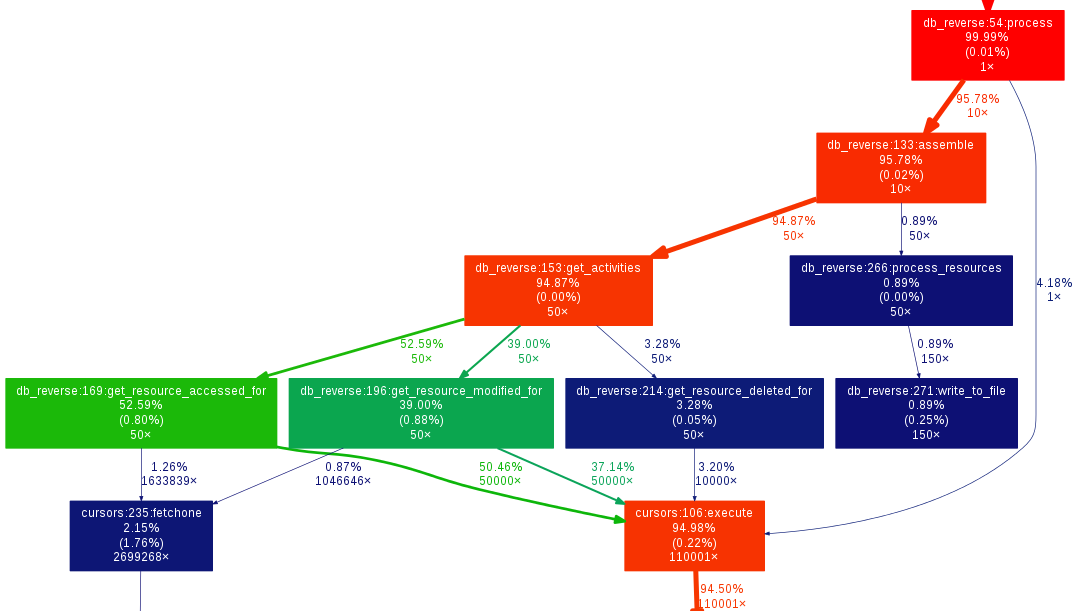
\includegraphics[scale=0.4]{figures/activities_creation.png}
% \end{center}
% \end{figure}
\\
\subsection{LDA Model}
\label{sub:LDA Model}
We used python module Gensim~\cite[Gensim]{gensim}  for the clustering and used the LDA multicore model which we described in~\autoref{ssub:Gensim}.
The LDA model generation code snippet is shown in~\autoref{lst:lda.py}.
The corpora consisted of one document per line.
We created a dictionary from the corpora using Gensim \emph{`corpora.Ditionary`} module~\cite[]{gensimdict}.
Dictionary is representation of all the unique tokens (words) by a unique token-ids.
We filtered the dictionary by discarding any resource activity that occurred in less than 10 or more than 1 million for clustering, as those activities are too less or too common to take into consideration.
% The lower and upper limit were chosen based the cumulative distribution function graph of resource activities.
We kept only $200,000$ tokens after the filtering.
This is done in line $7$~[\autoref{lst:lda.py}], where the arguments passed into \emph{`filter\_extremes'} method are minimum threshold (which is 10), maximum threshold in fraction (which is $0.14$: 1,000,000 out of total \gettotalmalwareiii{} documents), and total number of frequent words to keep after filtering (which is $200,000$).
In line 9--12~[\autoref{lst:lda.py}], we make an iterator to read the corpus.
The iterator operates on each line, which represents a document, of corpus text file and yields a bag of words of the document.
Bag of words is a list of two-element tuple, which represents word (token-id) and its count (number of occurrence) in document.
In line 15~[\autoref{lst:lda.py}], we create a LDA model for our corpus with 1000 topics.
The LDA gives the probability of different clusters that a document can belong to and we assign the document to the cluster with highest probability.\\
% The malware samples were clustered into 752 unique topics.
% This was based on heuristic after studying the cdf graph of activities to number of malware.
%TODO: add cdf of reverse index
% The number of topic was chosen to be 1000, however our malware samples were distributed among only 752 unique topic.
\begin{lstlisting}[float,floatplacement=H,language=python,caption={Script to run Gensim LDA},label={lst:lda.py}]
from gensim import corpora, models
import sys
document_name = sys.argv[1]
# read the file with malware activities and create dictionary
dictionary = corpora.Dictionary(line.split() for line in open(document_name))
# filter the dictionary for extreme
dictionary.filter_extremes(no_below=10,no_above=0.14,keep_n=1000000)
# create a iterator corpus as the file is large 80GB
class MyCorpus(object):
    def __iter__(self):
        for line in open(document_name):
            yield dictionary.doc2bow(line.split())

corpus = MyCorpus()
lda = models.ldamulticore.LdaMulticore(corpus=corpus,id2word=dictionary,num_topics=1000)
\end{lstlisting}

The number of clusters created were \textbf{``662''}.
The largest cluster size was {\getlargestclustersize{}} and the lowest was {\getlowestclustersize{}}.
The histogram and cumulative distributive graph showing the sizes of cluster can be seen in~\ref{fig:histclustersize},~\ref{fig:ecdfclustersize}, and~\ref{fig:cdfclusterlen}.
From the graph we can see that distribution of cluster size was mostly below 50,000.
$90\%$ of the cluster, about \emph{629 out of 662}, falls under the cluster size of less than 50,000.
Similarly, \emph{4 million} malware, which is the $65\%$ of total malware clustered, are in the cluster size of less than 50,000.\\

\begin{figure}[htbp]
\begin{center}
  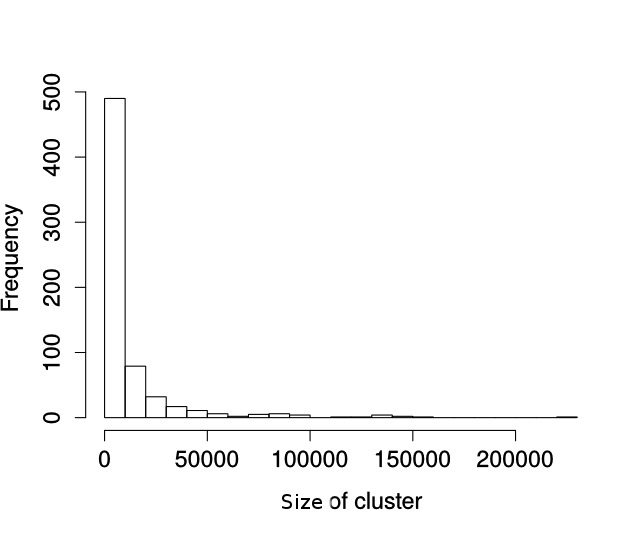
\includegraphics[scale=0.5]{figures/histclustersize_new.png}
\end{center}
\caption{Histogram showing the distribution of Cluster size}
\label{fig:histclustersize}
\end{figure}

\begin{figure}[htbp]
\begin{center}
  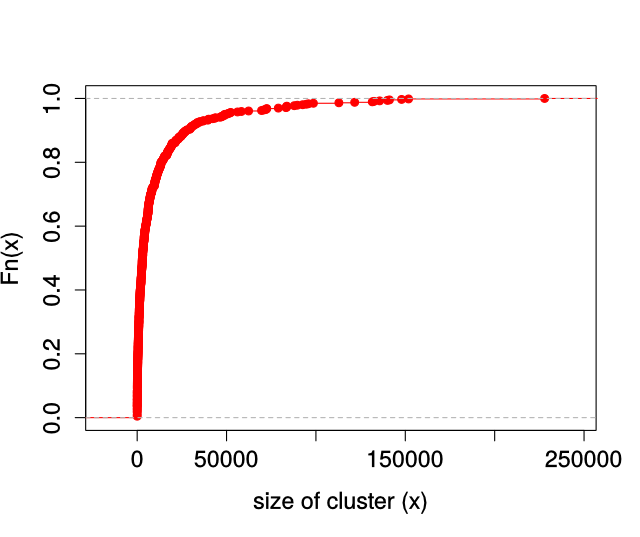
\includegraphics[scale=0.5]{figures/ecdfclustersize.png}
\end{center}
\caption{CDF between size of cluster and topic fraction}
\label{fig:ecdfclustersize}
\end{figure}

\begin{figure}[htbp]
\begin{center}
  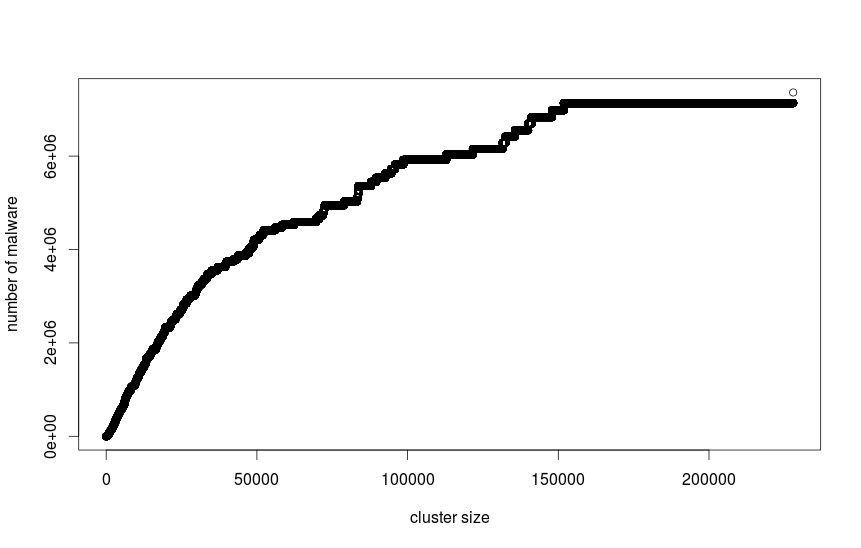
\includegraphics[scale=0.3,width=0.8\textwidth]{figures/cdfclusterlen2.png}
\end{center}
\caption{CDF between size of cluster and total number of malware}
\label{fig:cdfclusterlen}
\end{figure}
\subsection{Inter-Distance and Intra-Distance}
\label{sub:Inter-Distance and Intra-Distance}

We calculated the distance based on the average number of common words between the malware pair.
\textbf{Intra-distance} represents the average number of common words between the malware pair from same cluster.
\textbf{Inter-distance} represents the average number of common words between the malware pair from different clusters.
Since we want to cluster malware with similar behavioral activity together in same cluster; the intra-distance should be high (higher similarity among malware samples of same cluster), and the inter-distance should be low (lower similarity among malware samples from different cluster).
\\

To show the quality of our clustering we provide the following graph showing the graph of inter-cluster and intra-cluster distance in Figure~\ref{fig:intraclustcommon} and Figure~\ref{fig:interclustcommon}.\\
In case of intra-distance, for a cluster, we randomly selected 1000 malware pair (if possible because there were some clusters of size as small as 1), from the combinations of malware samples belonging to that cluster.
We calculated the average number of common resource activities\textit{(words)} present among the malware\textit{(document)} pair.
We can see that the average common words between the intra malware sample were good with intra-distance of at least \emph{500} covering $80\%$ of family topics~[\autoref{fig:intraclustcommon}].
For the inter-distance calculation, a cluster was paired with other clusters, and from those cluster pair,
we randomly selected 1000 malware pair (if possible because there were some clusters of size as small as 1).
We calculated the average common resource activities between those malware pairs to get the inter-distance.
We can see that the inter-distance of only 10 was covering almost $90\%$ of family topic~[\autoref{fig:interclustcommon}].
\begin{figure}[htbp]
\begin{center}
  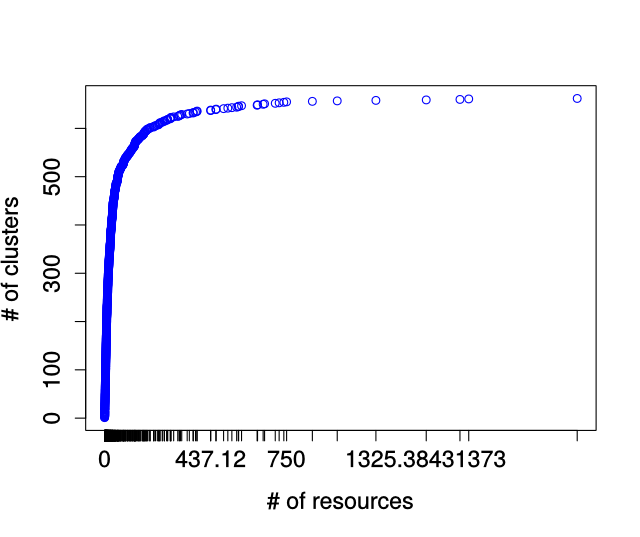
\includegraphics[scale=0.7]{figures/intra_clustered_common.png}
\end{center}
\captionsetup{font=small}
\caption{ Graph showing cdf distribution of common resource between same family topic}
\label{fig:intraclustcommon}
\end{figure}
\begin{figure}[htbp]
\begin{center}
  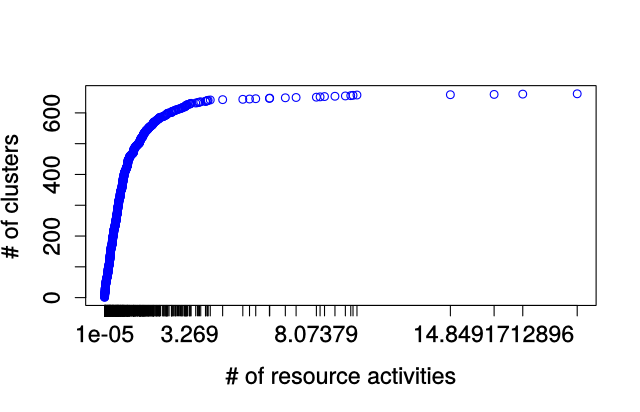
\includegraphics[scale=0.7]{figures/inter_clustered_common.png}
\end{center}
\captionsetup{font=small}
\caption{Graph showing cdf distribution of common resource between different family topic}
\label{fig:interclustcommon}
\end{figure}

\section{Finding Optimal Candidate Pairs}
\label{sec:Finding Optimal Candidate Pairs}
After the clustering, tens of thousands of malware associated with the resource, would now be reduced and represented by hundreds of families (clusters), that those malware belong to.
As described in~\autoref{sub:Candidate Selection}, we chose the candidate pair corresponding to a resource, such that each malware in the pair belongs to different clusters.
% We need to make sure that the family pair associated with the single resource is not repeated.
% We needed to further filter the candidate pairs, such that malware pair from same clusters, does not repeat for different resource name.
In order to find the optimal set of candidate pairs we interpreted the interaction of malware and resource, with respect to cluster, into Flow Network.
\subsection{Max Flow Approach}
\label{sub:Max Flow Approach}
We wanted to find the optimal pair of malware such that we have all the interesting mapped resource covered along with the cluster associated with it.
We represented the mapping between the resource, malware, and cluster as a flow network, and run the max flow algorithm as given in Figure~\ref{fig:maxflow}.\\

The network is made of 4 layers, other than sink and source.
Layer one is read/delete malware, the malware samples that tried to access or delete interesting resources but failed.
Layer two is combinations of clusters (\emph{ic=input-cluster}), that the malware with failed access or delete attempt belongs to, and the resource on which the malware tried to operate.
Layer three is the combinations of clusters (\emph{oc=output-cluster}), that the malware with successful modification operation belongs to, and the resource that they could successfully modify.
Layer four is the malware that successfully modified the resource.\\
The flow rules were:
\begin{itemize}
  \item All malware from layer one is connected from sources and also connected to the input cluster and resource combination it belongs to.
  \item All input-cluster and resource combination in layer two is connected to all output cluster resource combination in layer 3 that has a matching resource.
  \item All output-cluster and resource combination in layer 3 is connected to the corresponding malware in layer 4.
  \item Each malware in layer 4 is connected to the sink (T).
\end{itemize}
The capacities were:
\begin{itemize}
  \item All connections have capacity of infinite except connections from layer 2 to layer 3.
  \item All connections from layer 2 to layer 3 have a capacity of one.
\end{itemize}

\begin{figure}[htbp]
  \centering
  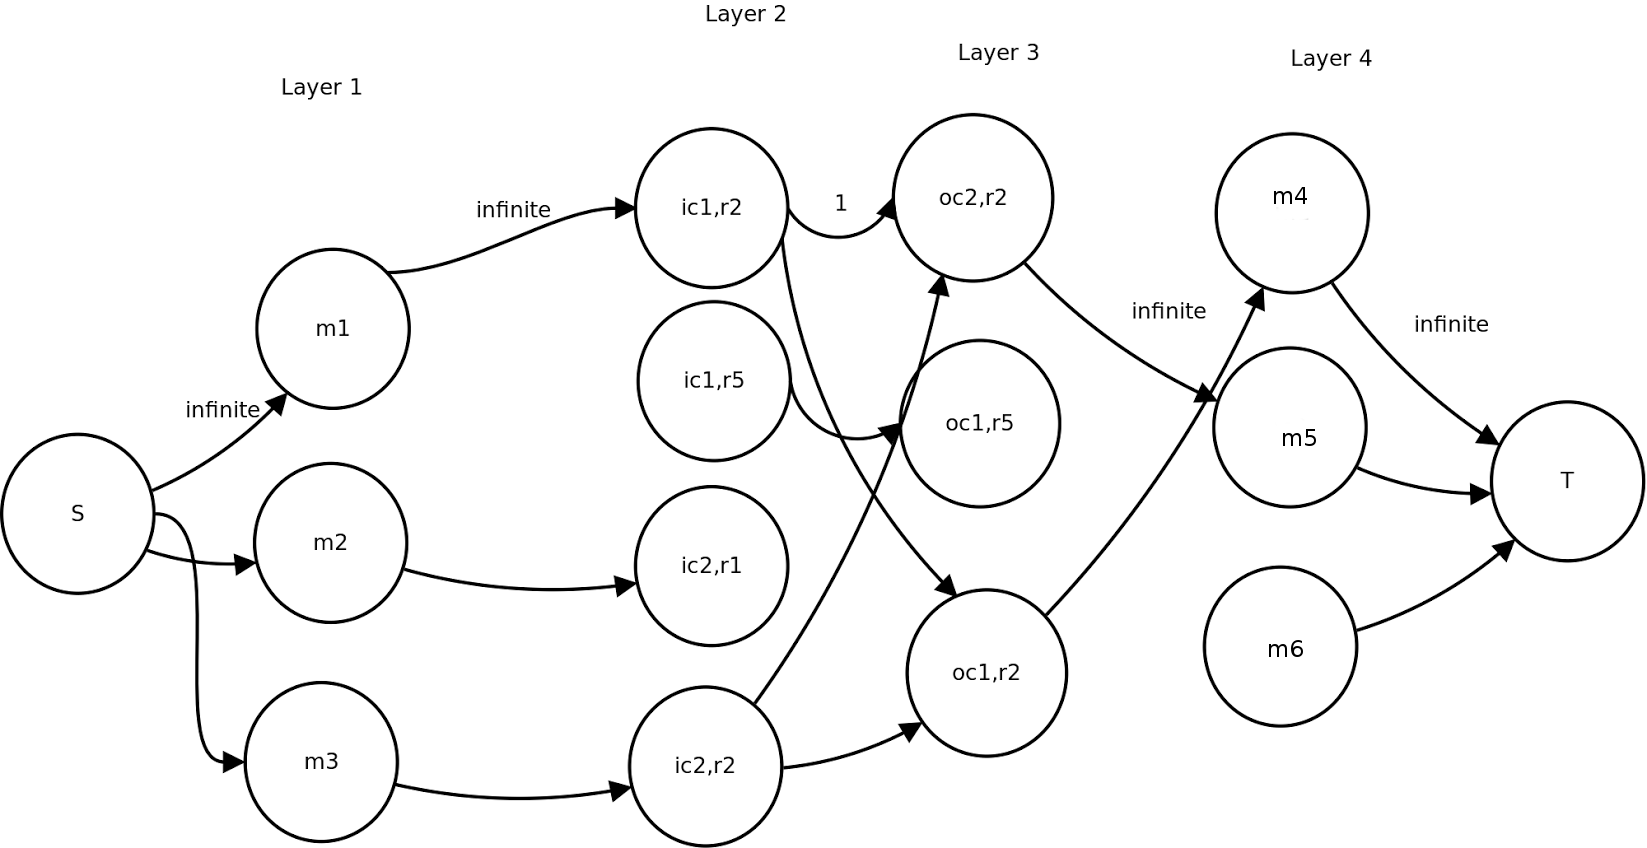
\includegraphics[scale=0.23]{figures/maxflow2.png}
  \caption[Max Flow]{Graph representing the max flow implementation}\label{fig:maxflow}
\end{figure}

The maximum flow in this network corresponds to an optimum match up.
To explain, in~\autoref{fig:maxflow}, `$m_1$' in layer 1 is connected to $(ic_1,r_2)$ in layer 2.
There are two cluster-resource combination, $(oc_2,r_2)$ and $(oc_1,r_2)$, in layer 3, that has resource `$r_2$' common with $(ic_1,r_2)$ cluster-resource combination.
So our candidate pairs would be, $(m_1,m_5)$ and $(m_1,m_4)$ operating on `$r_2$'.
Path from source (S) to $m_2$ in layer 1 and $(ic_2,r_1)$ in layer 2 does not reach the sink (T); hence, it is omitted.\\

%TODO: maxflow did not provide optimal
% The max flow approach, did lower
The max flow approach gave us optimal candidate pairs such that each pair of cluster is only covered once.
However, the approach did not take care of repetition of cluster pair corresponding to different resource.
% If malware pair $(m_1,m_2$) is associated with resource $(r_1,r_2,r_3)$, same candidate pairs gets repeated three times.
If malware $m_1$ is belongs to input cluster $ic_1$ and malware $m_2$ belongs to output cluster $oc_2$ and both are associated with resource $(r_1,r_2,r_3)$, same candidate pairs $(m_1,m_2)$, belonging to same cluster pair $(ic_1,oc_2)$, gets repeated three times.
% We wanted to group those repetition so that we get only single candidate pair $(m_1,m_2)$and analyze the behavioral interference they might have on different resources.
We wanted to group those repetition so that we get single candidate pair $(m_1,m_2)$ that covers the unique cluster pair $(ic_1,oc_2)$, for all its corresponding resources $(r_1,r_2,\ldots,r_n)$.
We used heuristics approach to eliminate those repetition.
\subsection{Heuristics Approach}
\label{sub:Heuristics Approach}
% We see in the first approach, we are not covering all resource interactions that were meticulously carved from millions of data points. 
The problem was to find the ``minimal set'' of malware pairs that covers all unique cluster (family) pairs (dictated by the set of all candidate pairs) and it also covers all resources that help build the candidate pairs, i.e., for each resource \emph{`r'} from resources \emph{`R'}, at least one malware pair from the final set should correspond the resource \emph{r}.\\

The relations has been represented in the graph below, where, \emph{I} is a set of input clusters from set \emph{`A'} and \emph{`O'} is the set of output clusters from set \emph{`B'}.
Set \emph{`A', `B'} are the sets of malware samples successfully modifying the resource and accessing/deleting the resource with failed attempt, respectively.
\emph{`R'} is the set of all interesting resources.
% They have also been described in the\textit{~\autoref{sub:Candidate Selection}}.
\begin{figure}[htbp]
  \centering
  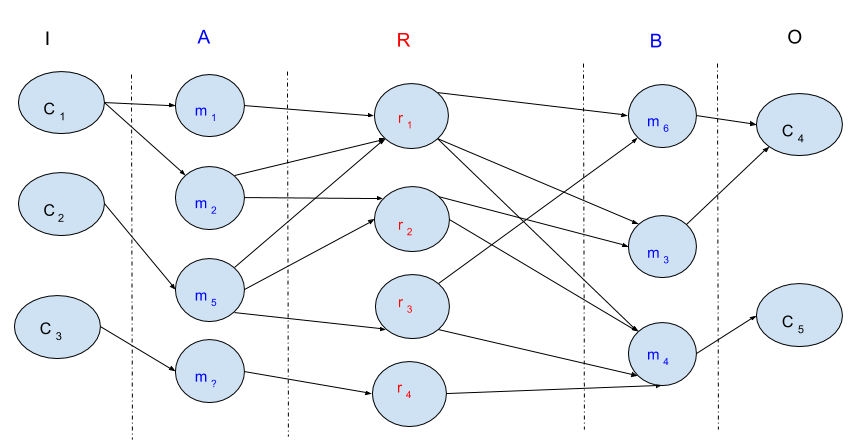
\includegraphics[scale=0.45]{figures/dhkheuristics.png}
  \caption[]{Heuristics approach to optimal malware pair selection}\label{fig:dhkheuristics}
\end{figure}
\\

In the Figure~\ref{fig:dhkheuristics},  $m_1,m_2, m_5$ samples create resource $r_1$, which is accessed (failed attempt) by $m_6, m_3$, and $m_4$.
The malware $m_1$ and $m_2$ maps to cluster $c_1$. Malware $m_6$ and $m_3$ maps to cluster $c_4$, and so on.
We need to find the minimal number of paths from each element \emph{$c_x$} of set \emph{`I'} to all reachable elements in \emph{`O'} (reachable from \emph{$c_x$}), such that all reachable elements \emph{`r'} in \emph{`R'} (reachable from \emph{$c_x$}) are traversed.
From such minimal set, we generated the candidate pairs by taking members of \emph{A} and \emph{B} from the path.
% This should work as we hard clusters (sample only falls into one cluster).
\\

We created the data structure as shown in~\ref{lst:dbdict}.
The data is a dictionary.
All candidate cluster pairs are keys and the value is a dictionary whose keys are malware pairs (all candidate malware pairs belonging to the cluster pair) and values are the list of corresponding resource.
\begin{lstlisting}[language=python,floatplacement=htpb,caption={Database Structure},label={lst:dbdict}]
db = { (c_i, c_o) :
    { (m_a, m_b) : [ r1, r2 ,...],
        ...,
     }
}
\end{lstlisting}
\begin{lstlisting}[float,floatplacement=htbp,language=python,caption={Pseudo code (Python) to get minimal set of candidates for all resource},label={lst:heuristicalgo}]
candidate_set = set()
for c_pair, v in db.iteritems():
    # reverse sort malware pairs by number of associated resources
    x = sorted( [(len(b), a) for a,b in v.iteritems()] , reverse=True)
    r_set = set()
    for c, m_pair in x:
        cur_r = v[m_pair]
        if not r_set.issuperset(cur_r):
            r_set = r_set.union(cur_r)
            candidate_set.add(m_pair)
\end{lstlisting}

The reduced candidate set was computed as shown in pseudo-code~\ref{lst:heuristicalgo}.
It is a greedy algorithm starting from the malware pair that corresponds most number of resource interactions.
For each malware pair it checks if that pair has been already chosen, and if not, adds the pair to the candidate list.
% \section{Testing the Candidate Pairs}
% \label{sec:Testing the Candidate Pairs}
